\chapter{Modelado de los datos: ordenación de los usuarios}
\label{chap:ordenacion_de_usuarios}

Una vez que ya tenemos una lista de usuarios cuyas publicaciones en Twitter
indican que podrían ser candidatos para las ofertas de trabajo, el siguiente
paso es ordenarlos de acuerdo a su relevancia. A continuación describimos brevemente
los dos criterios que usaremos para ordenarlos (el detalle de los algoritmos y 
procedimientos llevados a cabo en cada caso se hará en la secciones siguientes):
\begin{itemize}
\item Ordenación de tipo índice $h$. El índice h es un sistema propuesto por Jorge Hirsch, de la Universidad de California, para la medición de la calidad profesional de los científicos, en función de la cantidad de citas que han recibido sus artículos científicos\footnote{\url{https://en.wikipedia.org/wiki/H-index }}. Un científico tiene índice $h$ si ha publicado $h$ trabajos con al menos $h$ citas cada uno. El índice se diseñó para medir eficazmente la calidad del investigador, a diferencia de sistemas de medición más sencillos que cuentan citas o publicaciones, donde se hace una distinción entre aquellos investigadores que tienen una gran influencia en el mundo científico de aquellos que simplemente publican muchos trabajos. En nuestro campo, lo que queremos es medir 
la relevancia de los candidatos, así que una métrica de este tipo aplicada a los tuits publicados
de la temática de interés (Big Data y ciencia de datos en nuestro caso), nos ayudará a determinarla.
Los detalles, en la sección \ref{subsect:indice_h}.

\item Ordenación en función del papel de cada usuario dentro de la red de usuarios
seleccionados (sección \ref{subsect:grafo}). Para ello, construiremos el grafo 
de los candidatos y sus relaciones, siendo estas relaciones dirigidas (A está relacionado
con B si A sigue a B).
\end{itemize}

Con estos dos métodos pensamos que quedará bastante bien representado el panorama
de candidatos a partir de la información extraída de Twitter. 
Todos los cálculos descritos en esta parte del proyecto están en el archivo
{\bf user\_rank.py} del repositorio de GitHub.

En las siguientes seccies detallamos los algoritmos que hemos usado para cada sistema de
clasificación, aportando la justificación de las diversas elecciones que 
hemos llevado a cabo.

\section{Índice h}
\label{subsect:indice_h}
La particularización del índice $h$ a nuestro contexto podría ser 
del siguiente modo: un usuario de Twitter tendrá índice $h$ si $h$ de sus $N$ tuits
sobre un determinado tema, han sido retuiteados al menos $h$ veces.

Calcular el índice $h$ implica por tanto los siguientes pasos:
\begin{enumerate}
\item Explorar el timeline\footnote{\lq\lq Timeline\rq\rq es la palabra
que usan en Twitter para referirse a un flujo de publicaciones a lo largo del tiempo.
El timeline de un usuario es el flujo de las publicaciones de ese usuario.} 
de cada usuario. Para ello usaremos la función
{\tt user\_timeline} que ofrece el paquete de Python {\tt Tweepy}. 
\item Determinar, dentro de ese timeline, qué tuits son del tema que nos interesa
(Big Data o ciencia de datos) y descartar el resto.
\item De cada tuit publicado sobre el tema de interés, anotar su número de 
retuits y calcular el índice $h$. 
\end{enumerate}

La descarga del timeline de usuarios tienen varias limitaciones en el acceso a través 
del API de Twitter\footnote{\url{https://developer.twitter.com/en/docs/tweets/timelines/api-reference/get-statuses-user_timeline }}:
\begin{itemize} 
\item límite de $1500$ llamadas por cada ventana de $15$ minutos,
\item solo se permite acceder a los $3200$ más recientes tuits de cada usuario,
\item el número de tuits descargados en cada llamada al API solo puede ascender a $200$.
\end{itemize}
Para que el proceso de obtención de datos no se pare cuando alcanzamos el límite
de llamadas (da un error), la función de {\tt Tweepy} permite incluir el parámetro 
{\tt wait\_on\_rate\_limit = True} para gestionar ese error y esperar a reanudar
el proceso cuando sea posible.

La función del API de Twitter para obtener el timeline de los usuarios no tiene 
la opción de buscar tuits de forma temporal (por ejemplo, los de los tres
últimos meses). Hemos optado por evaluar el timeline respecto a los últimos
$200$ tuits publicados por parecernos un número lo suficientemente amplio para 
el objetivo de clasificar los usuarios, si bien se podría incluir en el código la
gestión de un número mayor de tuits en el timeline (aumentando el número de
llamadas al API).

Un aspecto importante a la hora de evaluar el impacto del usuario es distinguir 
entre sus publicaciones originales y los retuits. De los tuits que componen el 
timeline, vamos a extraer la siguiente información:
\begin{itemize}
\item el número de tuits descargados(que 
en principio serán $200$, pero podrían ser menos),
\item el número de tuits sobre el tema de interés, y por tanto el
porcentaje de tuits de interés sobre el total de tuits evaluados,
\item sobre los tuits de interés, el porcentaje de aquellos que son retuits,
\item el índice $h$ de los tuits originales. Para calcular el índice $h$ 
contaremos tanto las veces que se ha retuiteado el tuit como las que ha sido
citado.
\end{itemize}

Como información adicional también obtendremos el idioma en el que los usuarios han 
publicado los tuits. En esta parte del proyecto reutilizamos por tanto dos herramientas
mencionadas en la parte de selección de usuarios: el modelo que nos permite detectar si
un tuit es relevante o no (explicado en la sección \ref{sect:tuits_relevantes})
y el algoritmo para detectar el idioma de un texto (visto en la sección \ref{sect:deteccion_idioma}).

Al intentar bajar el timeline de algunos usuarios se pueden
obtener diversos mensajes de error (por ejemplo, porque el usuario tenga
protegido tu timeline, porque el usuario haya dejado de existir, etc.)
de forma que el proceso puede fallar. El código debe contemplar ese
caso y permitir que la ejecución continue con el resto de usuarios:

\myfigure{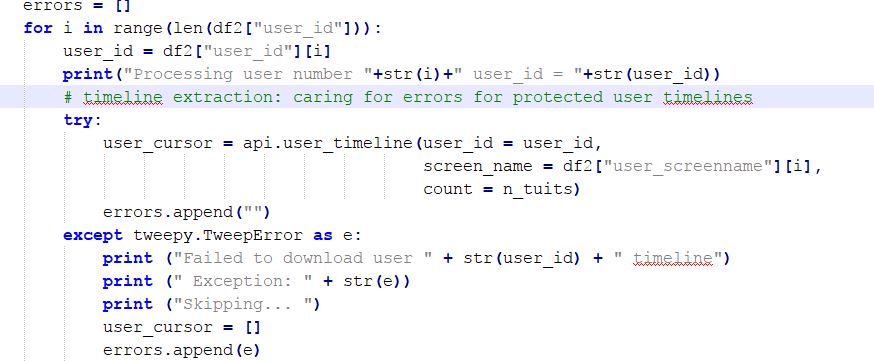
\includegraphics[width=0.6\textwidth]{error_not_authorized}%
\figcaption{Control de errores en la descarga de timelines.}
\label{fig:error_not_authorized} }


\section{Grafo relacional}
\label{subsect:grafo}
Nuestro objetivo en esta parte es explorar las relaciones entre los usuarios que 
hemos identificado como relevantes. De forma natural, como en cualquier red social,
se pueden definir multitud de estructuras de tipo grafo para describirlas. Nosotros
vamos a usar un grafo cuyos vértices serán los usuarios, y cuyas aristas o arcos serán
las relaciones entre ellos, de tipo dirigido: el usuario A está relacionado con el
usuario B si A sigue a B (y puede muy bien ocurrir que B no esté relacionado con A,
según esta definición). 

Para esta parte necesitaremos entonces descargar de Twitter la información
necesaria para construir el grafo de relaciones: los seguidores 
(\lq\lq followers\rq\rq\footnote{A aquellos usuarios que siguen a un determinado usuario, 
en Twitter se les denomina \lq\lq followers\rq\rq. Y se llaman \lq\lq friends\rq\rq aquellos
a los que dicho usuario determinado sigue.})
de cada uno de los usuarios identificados como potenciales candidatos. 
En principio, podríamos usar tanto los followers como los friends de cada uno 
de los usuarios de nuestra lista. Pero en realidad no hace falta, ya que si el usuario
A es un friend del usuario B, B es un follower del usario A, y lo consideraremos al
estudiar los followers de A. 

Para explorar los followers de cada usuario seleccionado usaremos la función 
{\tt followers\_ids} del paquete {\tt Tweepy}. Esta función es una interfaz
para la función del API de Twitter que permiten acceder a la lista de 
followers. Esta función del API de Twitter
tiene una limitación de $15$ llamadas al API por cada ventana de $15$ 
minutos\footnote{\url{https://developer.twitter.com/en/docs/accounts-and-users/follow-search-get-users/api-reference/get-followers-ids }},
con lo que la gestión de los límites es especialmente importante en este caso.
El parámetro {\tt wait\_on\_rate\_limit = True} al crear el acceso al API a 
través de {\tt Tweepy} también nos va a ser de utilidad.

Por otro lado, la información que puede descargarse con esa función también
está limitada en cantidad: el número de followers que puede obtenerse en cada llamada 
al API es a lo sumo $5000$. Igual que antes,
usando un código con varias llamadas al API, podríamos obtener un número más elevado de 
seguidores.

Nuestro grafo será por tanto un par ordenado 
$G=(N,g)$, donde $N$ es un conjunto de vértices o nodos, que serán los usuarios
identificados como potenciales candidatos para la oferta de trabajo, y $g$
es un conjunto de aristas o arcos, descritos como pares de nodos ordenados:
$$g=\{(a,b): a,b\in N, a \mbox{ sigue a }b\}.$$
En las representaciones de un grafo dirigido, una relación $(a,b)$ se 
suele describir con una flecha que sale de $a$ y apunta a $b$.
Al extraer la información sobre los usuarios hemos de quedarnos con los followers
de cada uno que están en el conjunto de usuarios, es decir, solo nos quedamos con
las relaciones entre candidatos:

\myfigure{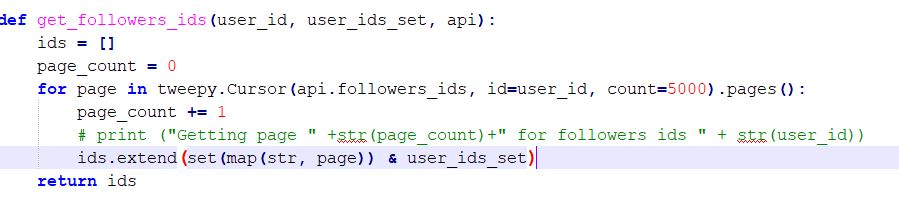
\includegraphics[width=0.8\textwidth]{followers_code}%
\figcaption{Followers y relación entre usuarios.}
\label{fig:followers_code} }

Una vez obtenidas estas relaciones, vamos a necesitar una librería 
para procesar el grafo y sacar las pertinentes 
conclusiones. A este respecto, tenemos varias opciones que 
considerar. Entre otras:
\begin{itemize}
\item {\tt Graph-tool}: los algoritmos están implementadas en una librería C++, 
lo que aporta mucha rapidez en la ejecución. Es 
buena procesando grafos grandes. La instalación en entornos Windows no
está soportada\footnote{\url{https://git.skewed.de/count0/graph-tool/wikis/installation-instructions 
}}.
\item {\tt NetworkX} es fácil de usar, para conjuntos de datos pequeños. Está bien
documentado. Es compatible con Python 2.7, 3.4, 3.5 y 3.6.
\item {\tt SNAP} (Stanford Network Analysis Platform): es un sistema para el análisis
y la manipulación de grandes redes. Está implementada en C++, con una interfaz en Python. 
Disponible para Python 2.7\footnote{\url{https://snap.stanford.edu/snappy/index.html }}.
\item {\tt igraph}: es una colección de herramientas para análisis de grafos,
con interfaces en R, Python y C/C++. Compatible con Python 2.6, 2.7 y 3.2.
\item {\tt APGL} (Another Python Graph Library): es una librería sencilla
para procesar grafos, disponible en principio para Python 2.7\footnote{\url{https://pythonhosted.org/apgl/ }}.
\end{itemize}

Vistas las opciones, nos hemos decidido por usar {\tt NetworkX}.
Esta herramienta nos va a permitir calcular varias métricas
que usaremos para estudiar el papel de cada usuario dentro de la red
y medir su relevancia (\cite{notas_fernando}, \url{https://www.sci.unich.it/~francesc/teaching/network/ }), y también explorar la estructura de la red, como exponemos a continuación.

\subsection{El papel de los usuarios: medidas de centralidad}

Las medidas de centralidad de los nodos de un grafo tratan de responder a la
cuestión de cuáles son los vértices más importantes o centrales dentro del 
grafo. La \lq\lq importancia\rq\rq de un nodo puede ser entendida 
de múltiples formas, y en consonancia hay diversas medidas de la misma.

Una vez que hemos determinado la medida de centralidad que nos interese para los nodos,
podremos usarla para ordenar la lista de los nodos (que es nuestro objetivo principal).

\subsubsection{Centralidad por grado}
El grado (degree) de un nodo $n$ es el número de aristas 
incidentes en $n$. En los grafos dirigidos podemos distinguir entre in-degree (número
de aristas que apuntan a $n$, en nuestro caso el número de followers) y
out-degree (número de aristas que parten de $n$, en nuestro caso, el número de
usuarios a los que sigue $n$). El in-degree representaría la capacidad de 
\lq\lq liderazgo\rq\rq
del usuario (a más followers, en principio más liderazgo), y el out-degree 
representaría el interés del usuario en seguir a otros usuarios, que podríamos
interpretar como su interés por el clima general del sector.

\subsubsection{Centralidad por autovector (eigenvector centrality)}
Es una extensión del 
concepto de cen\-tra\-li\-dad por grado que captura la intuición de que la importancia 
de un nodo en la red incrementa por el hecho de estar conectado a otros nodos 
a su vez relevantes. En un grafo dirigido, como el nuestro, parece natural pensar que
es más relevante la importancia de los usuarios que siguen a uno dado,
y que por tanto deberíamos usar los enlaces que apuntan al usuario en cuestion (las 
aristas que cuentan para el in-degree) para medir su propia importancia. 

Sea $c$ el vector columna
de las centralidades por autovector de los $N$ nodos del grafo y sea $A$ la matriz $N\times N$
de adyacencia del grafo, en la que $a_{ij}$ representa la contribución
del nodo $n_i$ al \lq\lq prestigio\rq\rq del nodo $n_j$ (en nuestro caso, $a_{ij} = 1$ si
$n_i$ sigue a $n_j$ y cero en caso contrario). La idea detrás de esta centralidad
(\cite{bonacich2}) es que la centralidad de un nodo será la suma de las centralidades
de los nodos que le apuntan, ponderadas por el peso de la unión, esto es:
$$c_i = \sum_j a_{ji} c_j$$
que en notación matricial es 
$$c = A^Tc.$$
Para asegurarnos de que esta ecuación tenga solución debemos considerar una formulación más general,
en la que la centralidad no es exactamente la suma de las centralidades de los nodos que 
contribuyen, sino solo un múltiplo de dicha suma:
$$\lambda c = A^Tc,$$
de tal forma que $c$, el vector de las centralidades del grafo es un 
autovector de la matriz $A^T$. Si $A$ es una matriz $N\times N$ hay en general $N$ soluciones
a dicha ecuación, correspondientes a los $N$ autovalores de $A^T$. Suele considerarse
como solución el autovector correspondiente al máximo autovalor.
 
La centralidad por autovector tiene un problema cuando
alguno de los nodos no tiene enlaces que lo apunten (es decir, si alguno de los usuarios
no tuviera ningún seguidor entre los demás usuarios, aunque él sí que siguiera a otros),
ya que en ese caso un nodo así siempre contribuirá cero, y por tanto, en algunos casos
la centralidad por autovector de todos los nodos sería cero:

\myfigure{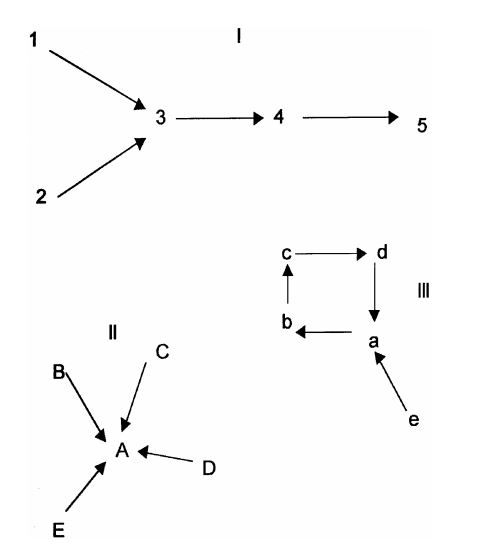
\includegraphics[width=0.6\textwidth]{grafos_bonacich}%
\figcaption{En los grafos I y II de estos ejemplos (extraídos de la página
192 de \cite{bonacich}), la centralidad por autovector de todos los nodos
es $0$.}
\label{fig:grafos_bonacich} }

Una medida de centralidad que puede ayudar en este tipo de situaciones es la 
centralidad de Bonacich.

% Dos medidas de centralidad que pueden ayudar en este tipo de situaciones son la 
% centralidad de Bonacich y la de Kleinberg.

\subsubsection{Centralidad de Bonacich}
Para paliar el problema mencionado anteriormente de la centralidad por 
autovector, podemos usar la centralidad de Bonacich, que  parte de la siguiente
idea: todos los nodos tienen una centralidad mínima. Con la misma notación que en el apartado
anterior, la centralidad de Bonacich puede definirse 
(ecuación $(5)$ en \cite{bonacich}) como:
$$c_i = e_i + \alpha\sum_j a_{ji} c_j, \mbox{ que en notación matricial es } c = e + \alpha A^Tc$$
donde $\alpha\in[0,1]$ y $e$ es un vector constante. Esto es, la centralidad de cada nodo es la suma
de una centralidad mínima (o exógena, como la denominan en \cite{bonacich}) 
y de las contribuciones a la centralidad de las centralidades de los nodos que apuntan 
a dicho nodo. Esa contribución se amortigua a través del parámetro $\alpha$, 
ya que para nodos a distancia $k$ de un nodo dado, su contribución es múltiplo de
$\alpha^k$. Si $\alpha=0$, no hay transmisión de centralidad.

% \subsubsection{Centralidad de Kleinberg}
% Hasta ahora, un nodo es importante si apuntan hacia él muchos nodos o si los nodos 
% que apuntan hacia él son importantes. Los nodos sin otros  nodos que apunten hacia 
% ellos, en el mejor de los casos cuentan
% con una centralidad mínima. Sin embargo, uno podría pensar que si un nodo apunta a otros nodos
% importantes, eso también debería ser importante. Por ejemplo, un artículo que cita a otros
% artículos importantes tiene el valor de indicarnos dónde encontrar información relevante y fiable.

% Podríamos entonces definir dos tipos de nodos: las autoridades (que contienen la información fiable)
% y los \lq\lq hubs\rq\rq, que nos dicen dónde está esa información fiable. La tesis de
% Kleinberg expuesta en \cite{kleinberg} es que un nodo es una autoridad si hacia él apuntan hubs,
% y es un hub si apunta hacia autoridades.

% La centralidad de Kleinberg también puede modificarse para incorporar una 
% centralidad exógena (como en la centralidad de Bonacich) o normalizar las centralidades
% de los nodos por su out-degree como en el PageRank.

% Sean $x$ e $y$ los vectores columna que denotan la centralidad por autoridad y por hub de
% los $N$ nodos del grafo. Con la misma notación que en los apartados anteriores, 
% se define la centralidad por autoridad $x_{i}$ como 
% $$x_i = \alpha  \sum_j a_{ji} \, y_j, \mbox{ o, en notación matricial, }x=\alpha  A^Ty,$$
% y la centralidad por hub como 
% $$y_i = \beta \sum_k a_{ij} \, x_j, \mbox{ esto es, } y =\beta A x,$$
% donde $\alpha$ y $\beta$ son dos constantes a determinar. Combinando las dos:
% \begin{eqnarray*}
% x & = &\alpha\beta A^T A x \\ 
% y & = &\alpha\beta A A^T y,
% \end{eqnarray*}
% y también
% $$ A x = \alpha\beta A A^T A x.$$ 
% Observemos que la matriz de autoridad $C = A^T A$ y la matriz de hub $R = A A^T$ tienen los
% mismos autovalores y que $y$ y $A x$ son dos autovectores de de la matriz de hub
% $R = A A^T$ con el mismo autovalor $1/\alpha\beta$. Entonces,
% una vez que calculamos el vector de centralidad por autoridad $x$, como 
% un autovector de la matriz de autoridad $C=A^TA$, podemos
% calcular la centralidad por hub como $y = A x$. En particular, la centralidad por hub
% del nodo $n_i$ es la suma de las centralidades por autoridad de los nodos que apuntan a $n_i$
% \footnote{La matriz $C$ se conoce como la matriz de co-citaciones
% en bibliometría: $C_{ij}=\sum_k a_{ki} a_{kj}$ es el número predecesores
% comunes de los nodos $n_i$ y $n_j$, y $C_{ii}$ es el in-degree de $n_i$. La matriz
% $R$ se conoce como la matriz de co-referencia en bibliometría: cada elemento 
% $R_{ij}=\sum_k a_{ik} a_{jk}$ es el número de sucesores comunes de $n_i$ y $n_j$, y 
% $R_{ii}$ es el out-degree de $n_i$. Esto da una interpretación alternativa de autoridades
% y hubs: un nodo es una autoridad si es muy co-citado con otras autoridades, y un nodo es un hub 
% si co-referencia a otros hubs.}.

\subsubsection{PageRank}
En las centralidades por autovector y de Bonacich, los nodos
distribuyen de forma indiscriminada su centralidad a todos los demás nodos a los que apunten, 
por lo que un nodo importante que apunta a muchos vecinos hace importantes a 
todos ellos. La idea de PageRank es repartir la centralidad aportada 
por un nodo entre todos aquellos a los que apunta, de tal forma que cada uno de ellos
recibirá solo la parte proporcional de la centralidad del nodo de partida, esto es,
la centralidad del nodo dividida por su out-degree (número de enlaces salientes):
$$c_i = (1-d) + d\sum_j a_{ji} \frac{c_j}{od(n_j)},$$
donde $od(n_j)$ es el out-degree del nodo $n_j$, y $d$ es un factor de amortiguación 
que tiene un valor entre 0 y 1. En la aplicación que hace Google de este algoritmo
(tienen una patente sobre él), parece que $d=0.85$, aunque la 
implementación concreta del algoritmo es por supuesto secreta. El papel de
$d$ es similar al de $\alpha$ en la centralidad de Bonacich, en
cuanto a la transmisión de la centralidad, y además ayuda a la convergencia
del cálculo del PageRank (se resuelve de forma iterativa).
En \cite{fdez} se puede encontrar una deliciosa explicación del algoritmo.

\subsubsection{Cercanía (closedness centrality)}
En un grafo conexo, la cercanía 
de un nodo es el inverso de la suma de las longitudes
de los caminos mínimos que unen dicho nodo con todos los demás:
$$c_i=\frac {1}{\sum _{j}d(n_j,n_i)},$$
donde $d(n_j,n_i)$ es la distancia geodésica\footnote{Las geodésicas son el camino
más corto entre dos puntos y no son necesariamente únicas.} 
entre los nodos $n_j$ y $n_i$. 

Cuanto más central es un nodo,
más cerca está del resto de nodos. Tales vértices pueden tener mejor acceso
a la información de otros nodos, o una influencia más directa en ellos. Por ejemplo, una persona
con mayor cercanía puede ver cómo sus opiniones alcanzan a otros usuarios más deprisa que 
las de alguien con menor cercanía. 

Frecuentemente, en lugar de la suma se considera la media de los caminos más cortos, 
de tal forma que se pueden comparar grafos de diferentes tamaños. Entonces, la formulación es:
$$c_i=\frac {N-1}{\sum _{j\neq i}d(n_j,n_i)},$$
donde $N$ es el número de nodos en el grafo. Si el grafo es muy grande, 
$N$ y $N-1$ son muy parecidos y suele usarse:  
$$c_i=\frac {N}{\sum _{j}d(n_j,n_i)}.$$
Considerar las distancias a o desde los otros nodos es irrelevante en grafos no dirigidos.
Pero en el caso de grafos dirigidos, puede producir resultados totalmente diferentes.
Cuando el grafo no es conexo, se puede usar la suma de los inversos de las distancias
en lugar del inverso de la suma de las distancias, con la convención 
$1/\infty =0$:
$$c_i=\sum _{j\neq i}\frac {1}{d(n_j,n_i)}.$$

\subsubsection{Intermediación (betweenness centrality)}
Captura en qué medida un nodo esta situado 
en los caminos que unen a otros nodos. Los nodos con una intermediación alta
pueden tener mucha influencia en la red, dado que \lq\lq controlan\rq\rq la información
que se transmite entre otros nodos. También son nodos que si desaparecieran impedirían
la transmisión de la información y aumentaría la desconexión de la red.

Matemáticamente, sea $n_{k,j}$ el número total de geodésicas que van desde $n_k$ a $n_j$,
y $n_{k,j}^{i}$ el número de ellas que pasan por $n_i$. Entonces, la
intermediación del nodo $n_i$ es:
$$c_i = \sum_{k,j} w_{k,j}^{i} = \sum_{k,j} \frac{n_{k,j}^{i}}{n_{k,j}},$$
donde el cociente $w_{k,j}^{i}$ expresa lo \lq\lq en medio\rq\rq que está $n_i$ de
$n_k$ y $n_j$, y por convención $w_{k,j}^{i} = 0$ si $n_{k,j} = 0$. 

Observemos que
la definición cuenta de forma distinta los caminos de $n_k$ a $n_j$ y de $n_j$ a $n_k$ 
(importante en grafos dirigidos), aquellos que empiezan o terminan en $n_i$ ($n_k=n_i$ o $n_j=n_i$) y también aquellos en los que $n_k=n_j$. Esto atiende al hecho de que parece razonable considerar
que un vértice está en medio cuando está en un camino entre él y algún otro, ya que en esos casos, también controla el flujo de información. En cualquier caso, usar otra definición no suele 
implicar mucha diferencia, ya que en general nos interesarán los valores relativos de la medida, y no
su valor absoluto. En ese sentido, suele normalizarse por el número total de pares ordenados
del grafo ($N^2$), para que la medida nos dé un número entre $0$ y $1$.

La tabla \ref{tab:medidas_cent_significado} resume las medidas de centralidad que vamos a incluir en nuestro análisis y una pequeña idea de su significado.

\begin{center}
\begin{table}
\begin{tabular}{c|c}
{\bf Centralidad} &{\bf Descripción}\\ \hline\hline
Por grado & Conexión total del usuario con la red\\ \hline
In-degree & Número de followers\\ \hline
Out-degree & Número de seguidos\\ \hline
Por autovalor & Importancia de los seguidores\\ \hline
Bonacich & Importancia de los seguidores más centralidad mínima\\ \hline
PageRank & Importancia proporcional de los seguidores más centralidad mínima\\ \hline
Cercanía & Facilidad de acceso a otros usuarios\\ \hline
Intermediación & Influencia y conexión de la red\\ \hline
\end{tabular}
\medskip
\caption{Medidas de centralidad e idea de su significado.}
\label{tab:medidas_cent_significado}
\end{table}
\end{center}

\subsection{La estructura de la red}
La teoría de grafos también nos permite extraer información
muy interesante sobre la estructura de la red de usuarios:
hay unas ciertas características que suelen aparecer en estructuras del
tipo que nos interesa, patrones que tienen un efecto importante en cómo 
se comportan estas redes.  Esta información no es directamente 
relevante para la ordenación de los usuarios, pero nos permitirá hacernos 
una idea más clara de cómo se organiza. Veamos algunas de dichas características.

\subsubsection{Estructura del grafo}
\begin{itemize}
\item Componentes conexas: una componente conexa de un grafo no dirigido es
un conjunto de nodos maximal (que no se pueden añadir más) tal que cualquier par de nodos
está conectado. Las componentes conexas son una partición del grafo (son disjuntas y
su unión es el grafo completo). En numerosos ejemplos reales, suele aparecer una gran
componente conexa (la componente gigante) que cuenta con una mayoría de los nodos (típicamente
más del $50$\%, pero no es infrecuente el $90$\%).  En los grafos dirigidos la noción de 
conectividad se complica y tenemos componentes débilmente conexas y fuertemente conexas:
	\begin{itemize}
	\item Dos nodos están en la misma componente débilmente conexa si están conectados por un camino,
	donde los caminos pueden recorrerse en cualquier sentido a lo largo de cualquier arista (esto es,
	como si el grafo fuera no dirigido).Se comporta igual que en el caso no dirigido, suele haber una
	componente gigante en la que se agrupan un alto porcentaje de los nodos.
	\item Dos nodos están en la misma componente fuertemente conexa si desde cada uno de ellos se puede
	ir al otro, a través de caminos dirigidos. Las componentes fuertemente conexas también
	forman una partición del grafo, y también se puede presentar una componente gigante,
	aunque debido a las restricciones del grafo, no suele ser tan grande. 
	\end{itemize}

\item Caminos mínimos (geodésicas)
	\begin{itemize}
	\item La excentricidad de un nodo en un grafo conexo es la mayor distancia
	geodésica entre ese nodo y cualquier otro vértice del grafo. En un grafo disconexo,
	o bien todos los nodos se definen con una excentricidad infinita, o bien se calcula 
	la excentricidad en la componente conexa a la que pertenezca el nodo. 
	\item Diámetro: la mayor distancia geodésica dentro del grafo (o componente si no es conexo). 
	Es la máxima excentricidad.
	\item Radio: la mínima distancia geodésica dentro del grafo.
	\item Longitud del camino medio: media de todos los caminos mínimos entre los 
	nodos del grafo (menos sensible a valores extremos).
	\end{itemize}
\item Distribución del grado de los nodos: del grado, out-degree o in-degree, da una idea
de lo conectada que está la red. La distribución conjunta del in y el out-degree
nos proporciona información sobre la correlación entre ambas cantidades. En muchos casos,
estas distribuciones suelen ser muy asimétricas: muchos nodos con valores bajos, y unos pocos
con valores muy altos.

\item Transitividad: Tres nodos $n_1, n_2, n_3$ tales que $n_2$ está relacionado con $n_1$ y $n_3$ forman un triángulo centrado en $n_2$.
El triángulo es cerrado si $n_1$ está relacionado con $n_3$, y abierto en caso contrario. La
transitividad mide la capacidad de la red para que los triángulos sean cerrados, esto es,
si un nodo $n_1$ está conectado
con otro nodo $n_2$, y éste con un tercero $n_3$, entonces $n_1$ también está conectado
con $n_3$.  
El coeficiente de transitividad de una red, también conocido
como coeficiente de clusterización, es el cociente entre el número de triángulos 
cerrados en la red, respecto al número de posibles triángulos. Las redes sociales
tienden a tener valores altos de transitividad\footnote{\cite{notas_fernando}, \url{https://www.sci.unich.it/~francesc/teaching/network/transitivity.html }:
por ejemplo, la transitividad de la colaboración entre autores en ciencias
de la computación es $0.24$, la de la red de colaboración entre actores
$0.2$ y la de coautores en publicaciones de física, $0.45$. Sin embargo,
la de Internet es solo $0.012$.}.
En las redes dirigidas, la transitividad se calcula como para las no dirigidas,
ignorando la dirección de las aristas.
\end{itemize}


\subsubsection{Grupos de nodos}
Desde el punto de vista de nuestra aplicación, podría ser interesante
descubrir, a través del estudio de la red, los grupos que pudieran formarse
entre usuarios. Estos grupos podrían deberse a agrupaciones de usuarios en
función de similares intereses, y detectar a través de ellos la especialización
de perfiles. Por ejemplo, es razonable pensar que alguien interesado en visualización
de datos, seguirá o será seguido por usuarios cuyo perfil también incluya un
interés en visualización de datos. 

Esta parte, sin embargo, requeriría un estudio muy detallado de la estructura
de la red, que no es el objetivo principal del proyecto.

\section{Almacenamiento}

